% Options for packages loaded elsewhere
\PassOptionsToPackage{unicode}{hyperref}
\PassOptionsToPackage{hyphens}{url}
%
\documentclass[
  ignorenonframetext,
]{beamer}
\usepackage{pgfpages}
\setbeamertemplate{caption}[numbered]
\setbeamertemplate{caption label separator}{: }
\setbeamercolor{caption name}{fg=normal text.fg}
\beamertemplatenavigationsymbolsempty
% Prevent slide breaks in the middle of a paragraph
\widowpenalties 1 10000
\raggedbottom
\setbeamertemplate{part page}{
  \centering
  \begin{beamercolorbox}[sep=16pt,center]{part title}
    \usebeamerfont{part title}\insertpart\par
  \end{beamercolorbox}
}
\setbeamertemplate{section page}{
  \centering
  \begin{beamercolorbox}[sep=12pt,center]{part title}
    \usebeamerfont{section title}\insertsection\par
  \end{beamercolorbox}
}
\setbeamertemplate{subsection page}{
  \centering
  \begin{beamercolorbox}[sep=8pt,center]{part title}
    \usebeamerfont{subsection title}\insertsubsection\par
  \end{beamercolorbox}
}
\AtBeginPart{
  \frame{\partpage}
}
\AtBeginSection{
  \ifbibliography
  \else
    \frame{\sectionpage}
  \fi
}
\AtBeginSubsection{
  \frame{\subsectionpage}
}

\usepackage{amsmath,amssymb}
\usepackage{iftex}
\ifPDFTeX
  \usepackage[T1]{fontenc}
  \usepackage[utf8]{inputenc}
  \usepackage{textcomp} % provide euro and other symbols
\else % if luatex or xetex
  \usepackage{unicode-math}
  \defaultfontfeatures{Scale=MatchLowercase}
  \defaultfontfeatures[\rmfamily]{Ligatures=TeX,Scale=1}
\fi
\usepackage{lmodern}
\ifPDFTeX\else  
    % xetex/luatex font selection
\fi
% Use upquote if available, for straight quotes in verbatim environments
\IfFileExists{upquote.sty}{\usepackage{upquote}}{}
\IfFileExists{microtype.sty}{% use microtype if available
  \usepackage[]{microtype}
  \UseMicrotypeSet[protrusion]{basicmath} % disable protrusion for tt fonts
}{}
\makeatletter
\@ifundefined{KOMAClassName}{% if non-KOMA class
  \IfFileExists{parskip.sty}{%
    \usepackage{parskip}
  }{% else
    \setlength{\parindent}{0pt}
    \setlength{\parskip}{6pt plus 2pt minus 1pt}}
}{% if KOMA class
  \KOMAoptions{parskip=half}}
\makeatother
\usepackage{xcolor}
\newif\ifbibliography
\setlength{\emergencystretch}{3em} % prevent overfull lines
\setcounter{secnumdepth}{-\maxdimen} % remove section numbering


\providecommand{\tightlist}{%
  \setlength{\itemsep}{0pt}\setlength{\parskip}{0pt}}\usepackage{longtable,booktabs,array}
\usepackage{calc} % for calculating minipage widths
\usepackage{caption}
% Make caption package work with longtable
\makeatletter
\def\fnum@table{\tablename~\thetable}
\makeatother
\usepackage{graphicx}
\makeatletter
\def\maxwidth{\ifdim\Gin@nat@width>\linewidth\linewidth\else\Gin@nat@width\fi}
\def\maxheight{\ifdim\Gin@nat@height>\textheight\textheight\else\Gin@nat@height\fi}
\makeatother
% Scale images if necessary, so that they will not overflow the page
% margins by default, and it is still possible to overwrite the defaults
% using explicit options in \includegraphics[width, height, ...]{}
\setkeys{Gin}{width=\maxwidth,height=\maxheight,keepaspectratio}
% Set default figure placement to htbp
\makeatletter
\def\fps@figure{htbp}
\makeatother

\makeatletter
\@ifpackageloaded{caption}{}{\usepackage{caption}}
\AtBeginDocument{%
\ifdefined\contentsname
  \renewcommand*\contentsname{Table of contents}
\else
  \newcommand\contentsname{Table of contents}
\fi
\ifdefined\listfigurename
  \renewcommand*\listfigurename{List of Figures}
\else
  \newcommand\listfigurename{List of Figures}
\fi
\ifdefined\listtablename
  \renewcommand*\listtablename{List of Tables}
\else
  \newcommand\listtablename{List of Tables}
\fi
\ifdefined\figurename
  \renewcommand*\figurename{Figure}
\else
  \newcommand\figurename{Figure}
\fi
\ifdefined\tablename
  \renewcommand*\tablename{Table}
\else
  \newcommand\tablename{Table}
\fi
}
\@ifpackageloaded{float}{}{\usepackage{float}}
\floatstyle{ruled}
\@ifundefined{c@chapter}{\newfloat{codelisting}{h}{lop}}{\newfloat{codelisting}{h}{lop}[chapter]}
\floatname{codelisting}{Listing}
\newcommand*\listoflistings{\listof{codelisting}{List of Listings}}
\makeatother
\makeatletter
\makeatother
\makeatletter
\@ifpackageloaded{caption}{}{\usepackage{caption}}
\@ifpackageloaded{subcaption}{}{\usepackage{subcaption}}
\makeatother

\ifLuaTeX
  \usepackage{selnolig}  % disable illegal ligatures
\fi
\usepackage{bookmark}

\IfFileExists{xurl.sty}{\usepackage{xurl}}{} % add URL line breaks if available
\urlstyle{same} % disable monospaced font for URLs
\hypersetup{
  hidelinks,
  pdfcreator={LaTeX via pandoc}}


\author{}
\date{}

\begin{document}


\begin{frame}{}
\phantomsection\label{section}
\end{frame}

\begin{frame}{Definition and milestones}
\phantomsection\label{definition-and-milestones}
\begin{itemize}
\tightlist
\item
  \textbf{Business model}: A business model describes the rationale of
  how an organization creates, delivers, and captures value.
\item
  Milestones in this century:

  \begin{itemize}
  \tightlist
  \item
    \textbf{2004}: Alexander Osterwalder introduces the Business Model
    Canvas.
  \item
    \textbf{2010}: Business Model Generation book is published.
  \item
    \textbf{2015}: Business Model Navigator book is published.
  \end{itemize}
\item
  Software

  \begin{itemize}
  \tightlist
  \item
    \href{https://businessmodelnavigator.com/}{Business model navigator}
  \item
    \href{https://www.strategyzer.com/library/the-business-model-canvas}{Strategyzer's
    Business Model Canvas}
  \end{itemize}
\end{itemize}
\end{frame}

\begin{frame}{Business model canvas}
\phantomsection\label{business-model-canvas}
\begin{center}
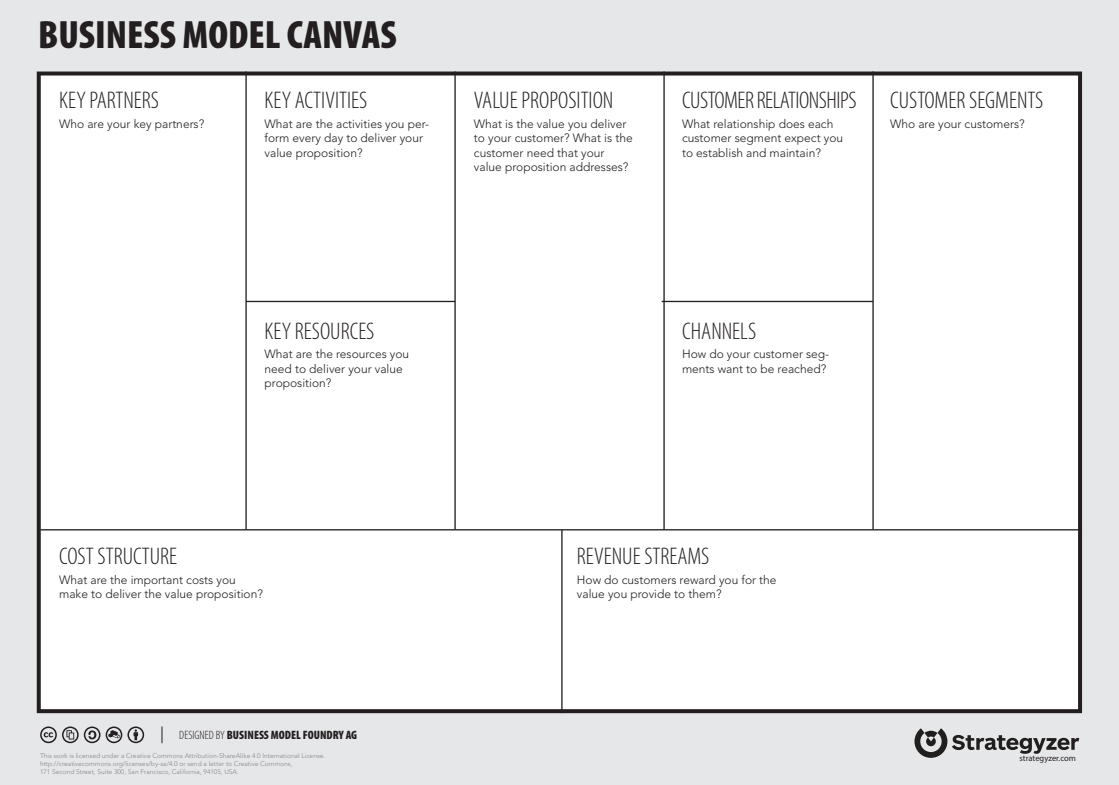
\includegraphics{figures/business_model_canvas.png}
\end{center}
\end{frame}

\begin{frame}{Business models extensions}
\phantomsection\label{business-models-extensions}
\end{frame}

\begin{frame}{Tripple layer business model (Joyce and Paquin, 2016)}
\phantomsection\label{tripple-layer-business-model-joyce-and-paquin-2016}
\begin{center}
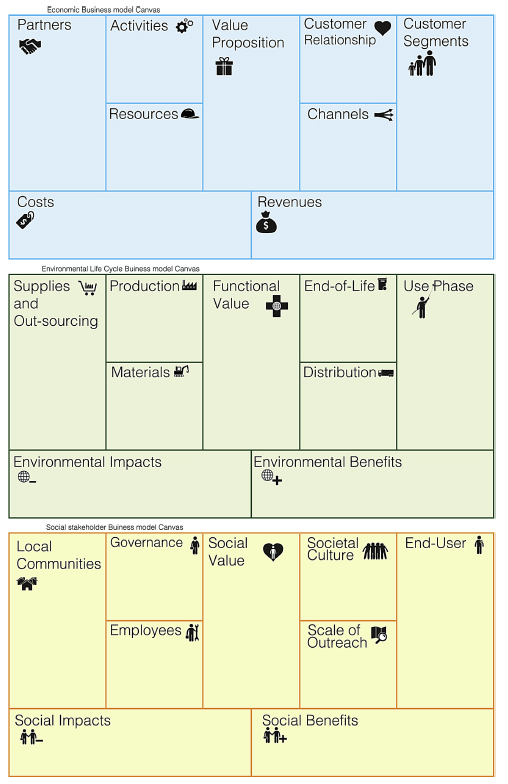
\includegraphics{figures/Triple-Layered-Business-Model-Canvas-TLBMC-image-from-Joyce-and-Paquin-2016.png}
\end{center}
\end{frame}

\begin{frame}{Threebility (Gerlach, 2015)}
\phantomsection\label{threebility-gerlach-2015}
\begin{center}
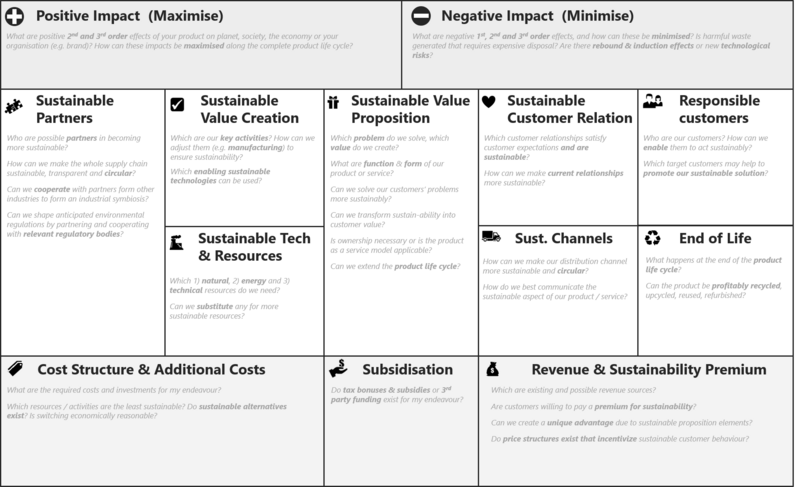
\includegraphics{figures/csm_mm1_Threebility_The_Sustainable_Business_Model_Canvas_03146e7333.png}
\end{center}

\note{\begin{itemize}
\tightlist
\item
  \textbf{Triple layer business model}: Focuses on the value
  proposition, value creation, and value capture layers.
\item
  \textbf{Threebility}: Adds a sustainability layer to the traditional
  Business Model Canvas.
\end{itemize}}
\end{frame}

\begin{frame}{ProGlreg business model (2023)}
\phantomsection\label{proglreg-business-model-2023}
\begin{center}
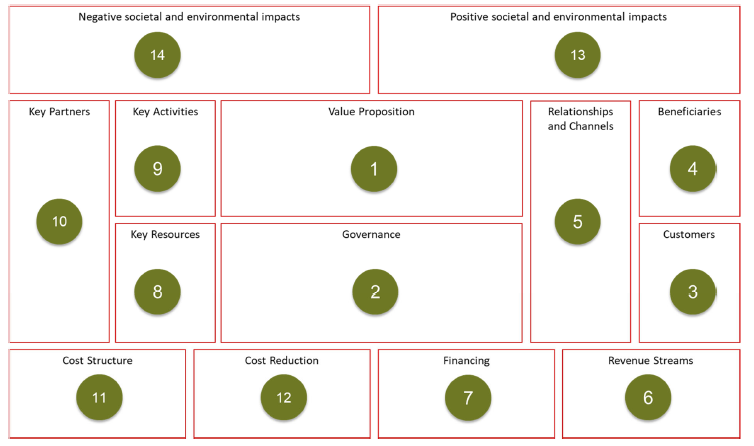
\includegraphics{figures/proGIreg_business_model_.png}
\end{center}
\end{frame}

\begin{frame}{ISO 59010 circular economy (2024)}
\phantomsection\label{iso-59010-circular-economy-2024}
\begin{center}
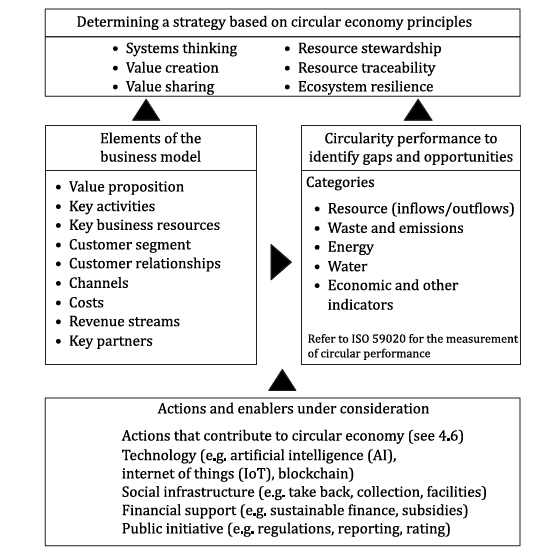
\includegraphics{figures/iso_59010_bm_circular_economy.png}
\end{center}
\end{frame}

\begin{frame}{Interviews and surveys following BS}
\phantomsection\label{interviews-and-surveys-following-bs}
\end{frame}

\begin{frame}{MD demo example}
\phantomsection\label{md-demo-example}
\end{frame}

\begin{frame}{Value Proposition}
\phantomsection\label{value-proposition}
\begin{itemize}
\tightlist
\item
  \textbf{Increasing biodiversity}: Bringing back native species and
  improving wetlands through water management and the green hatchery.
\item
  \textbf{Climate Resilience}: Carbon sequestration and improving water
  quality.
\item
  \textbf{Sustainable Development in NBS}: Promoting regenerative
  tourism, sports fisheries, and community involvement in restoration
  efforts.
\end{itemize}
\end{frame}

\begin{frame}{Key Partners}
\phantomsection\label{key-partners}
\begin{itemize}
\tightlist
\item
  \textbf{Croatian Waters (HRVODE)}: Hydrological works and floodplain
  restoration.
\item
  \textbf{University of Zagreb (UZ-FSB)}: Technology development and
  digital platform management.
\item
  \textbf{CEKOM}: Data collection and strategy development.
\item
  \textbf{Local and Regional Authorities}: Coordination of on-ground
  activities.
\item
  \textbf{NGOs and SMEs}: Supporting community engagement and
  eco-tourism.
\end{itemize}
\end{frame}

\begin{frame}{Key Resources}
\phantomsection\label{key-resources}
\begin{itemize}
\tightlist
\item
  \textbf{Natural Resources}: Wetlands and native fish species.
\item
  \textbf{Human Resources}: Biodiversity experts, local labor, and
  scientific researchers.
\item
  \textbf{Technological Resources}: Centralized data repository and
  monitoring tools.
\item
  \textbf{Financial Resources}: EU Horizon Europe funding.
\item
  \textbf{Green Hatchery Infrastructure}: Aquaculture systems with
  renewable energy sources.
\end{itemize}
\end{frame}

\begin{frame}{Key Activities}
\phantomsection\label{key-activities}
\begin{itemize}
\tightlist
\item
  \textbf{Hydrological Restoration}: Removing barriers and improving
  water flows.
\item
  \textbf{Green Hatchery Operations}: Cultivating native fish species.
\item
  \textbf{Biodiversity Monitoring}: Digital tools for tracking
  ecological health.
\item
  \textbf{Community Engagement}: Workshops, citizen science, and local
  job creation.
\item
  \textbf{Sustainable Aquaculture}: Long-term fishery management and
  economic development.
\end{itemize}
\end{frame}

\begin{frame}{Customer Segments}
\phantomsection\label{customer-segments}
\begin{itemize}
\tightlist
\item
  \textbf{Local Communities}: Benefiting from restored ecosystems and
  new economic opportunities.
\item
  \textbf{Regional and National Authorities}: Supporting environmental
  and flood management policies?
\item
  \textbf{Environmental Agencies}: Using the DEMO as a model for wetland
  restoration.
\item
  \textbf{Regenerative tourism community}: Leveraging the restored
  ecosystems for sustainable tourism.
\end{itemize}
\end{frame}

\begin{frame}{Channels}
\phantomsection\label{channels}
\begin{itemize}
\tightlist
\item
  \textbf{Digital Platforms}: Website, social media (Facebook, YouTube),
  and newsletters.
\item
  \textbf{Community Events}: Workshops, and participatory monitoring.
\item
  \textbf{Printed Materials}: Flyers, posters, and press releases.
\item
  \textbf{International Conferences}: Sharing knowledge with the broader
  scientific and policy communities.
\item
  \textbf{Portal} - Centralized data repository and monitoring tools.
\end{itemize}
\end{frame}

\begin{frame}{Revenue Streams}
\phantomsection\label{revenue-streams}
\begin{itemize}
\tightlist
\item
  \textbf{Regenerative Tourism and Sports Fisheries}: Income from guided
  tours, fishing permits, and eco-lodging.
\item
  \textbf{Sustainable Aquaculture}: Sale of native fish species to local
  markets.
\item
  \textbf{Reed and Plant Harvesting}: Sustainable use of wetland plants
  for bio-based materials.
\item
  \textbf{Environmental Consulting}: Offering expertise in wetland
  restoration to other regions.
\item
  \textbf{Data API} - subscriptoin on the portal?
\end{itemize}
\end{frame}

\begin{frame}{Cost Structure}
\phantomsection\label{cost-structure}
\begin{itemize}
\tightlist
\item
  \textbf{Restoration Costs}: Hydrological engineering, hatchery
  operations, and maintenance.
\item
  \textbf{Technology and Monitoring}: Sensors, drones, and data
  management systems.
\item
  \textbf{Community Engagement}: Workshops, educational programs, and
  local involvement.
\item
  \textbf{Project Management}: Administrative costs, legal compliance,
  and project coordination.
\end{itemize}
\end{frame}

\begin{frame}{Data and tools for dynamic reporting and interactivity}
\phantomsection\label{data-and-tools-for-dynamic-reporting-and-interactivity}
\end{frame}

\begin{frame}{Data Used in Business Model Preparation}
\phantomsection\label{data-used-in-business-model-preparation}
\begin{itemize}
\tightlist
\item
  \textbf{Environmental Data} - water quality, biodiversity indicators,
  carbon sequestration data.
\item
  \textbf{Socio-economic Data} - macro data, local employment, business
  subject dynamics.
\item
  \textbf{Community and Stakeholder Feedback} - community surveys,
  interviews.
\end{itemize}
\end{frame}

\begin{frame}{Data Science principles}
\phantomsection\label{data-science-principles}
\begin{itemize}
\tightlist
\item
  \textbf{Dynamic} - automatic updates when new data is ingested or
  parameters are changed.
\item
  \textbf{Interactive} - allow users to explore data and insights.
\item
  \textbf{Reproducible} - analyses should be reproducible by other teams
  using the same datasets and methods.
\item
  \textbf{Automated Data Pipelines} - automate data collection,
  cleaning, and reporting to ensure consistent updates.
\item
  \textbf{Versioning and Traceability} - track all changes to data,
  code, and reports to ensure they can be replicated or rolled back.
\item
  \textbf{Open source} - use open-source tools and libraries to ensure
  transparency and collaboration.
\item
  \textbf{Example} - \href{https://forensis.shinyapps.io/dawetrest/}{MD
  Demo business model}
\end{itemize}
\end{frame}

\begin{frame}{}
\phantomsection\label{section-1}
\end{frame}




\end{document}
